\begin{frame}[plain,c]
\begin{center}
	\huge Important remark
\end{center}
\end{frame}

\begin{frame}
	\pause[1]
	\begin{theorem}
		If a $(v,k,\lambda)-BIBD$ exist, then $\lambda(v-1) \equiv 0 (mod(k-1))$ and $\lambda v(v-1) \equiv (mod k(k-1))$.
	\end{theorem}
	
	\pause[2]
	Only \textbf{necessary}.
	
	\pause[1]
	\begin{theorem}
		A STS of \textit{order} $v$ \textbf{exists} if and only if $v\equiv 1,3\ mod(6)$  
	\end{theorem}
	
	\pause[2]
	\textbf{Necessary} and \textbf{sufficient}.
\end{frame}
\begin{frame}
\frametitle{STS on OEIS}
\begin{figure}
	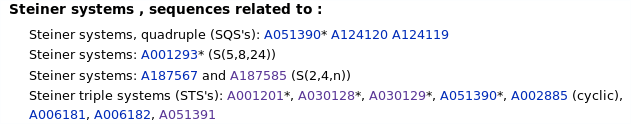
\includegraphics[width=1\textwidth]{oeis_on_sts}
\end{figure}
\end{frame}

\begin{frame}
\frametitle{Isomorphisms between two \textit{design}}
\begin{block}{Isomorphism}
Two designs $(X,\mathrm{A})$ and $(Y,\mathrm{B})$ where $|X|=|Y|$ are \textit{isomorphic} if there \textit{exists} a bijection $\alpha : X \rightarrow Y$ such that:
\begin{center}
	\begin{math}
	[ \{ \alpha(x) : x \in A \}: A \mathrm{A} ] = \mathrm{B}
	\end{math}%In other words, if we rename every point x ∈ X by α(x), then the collection of blocks
	% is transformed into B. The bijection α is called an isomorphism.

\end{center}
Then $\alpha$ is called isomorphism.
\end{block}
\begin{figure}
	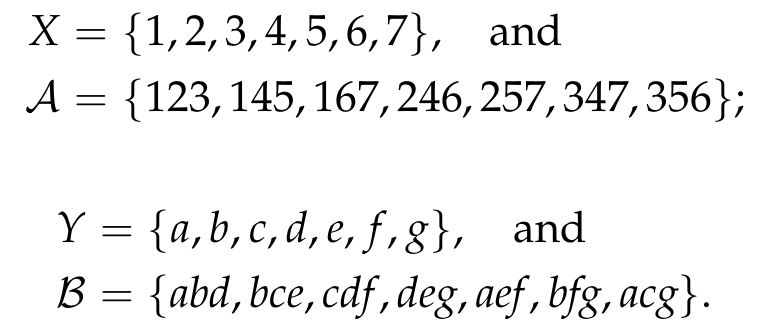
\includegraphics[width=0.65\textwidth]{isomorphism}
\end{figure}
\end{frame}

%due sts non-isomorfi quindi sono sts che hanno lo stesso ordine ma che una funzione biunivoca non riesce a mappare, effettivamente sono diversi quindi.
\begin{frame}
\frametitle{Beyond Existence or non-existence}

\setbeamercolor{block title}{bg=red!30,fg=black}

\pause[1]
\begin{block}{}
The existence of non-isomorphic STS is complex and a open field.
\end{block}


\setbeamercolor{block title}{bg=blue!30,fg=black}
\pause[2]
\begin{block}{(A030129) Number of nonisomorphic Steiner triple systems (STS's) $S(2,3,n)$ on $n$ points}
	$<1, 0, 1, 0, 0, 0, 1, 0, 1, 0, 0, 0, 2, 0, 80, 0, 0, 0, 11084874829>$%fino a 19 e il primo che ne ha 2 è 9
\end{block}
\begin{block}{(A051390)Number of nonisomorphic Steiner quadruple systems (SQS's) of order $n$ }
	$<1, 1, 0, 1, 0, 0, 0, 1, 0, 1, 0, 0, 0, 4, 0, 1054163>$%16
\end{block}
\end{frame}